% Chapter 3
\chapter{Monitored Building Dataset} % Main chapter title
\label{Chapter3} % For referencing the chapter elsewhere, use \ref{Chapter2} 
\minitoc
%----------------------------------------------------------------------------------------

%% Define some commands to keep the formatting separated from the content 
%\newcommand{\keyword}[1]{\textbf{#1}}
%\newcommand{\tabhead}[1]{\textbf{#1}}
%\newcommand{\code}[1]{\texttt{#1}}
%\newcommand{\file}[1]{\texttt{\bfseries#1}}
%\newcommand{\option}[1]{\texttt{\itshape#1}}

%----------------------------------------------------------------------------------------

This chapter is devoted to the description of the multivariate building dataset and the way in which we manage the time series data. The first section describes the provided raw data, the next section describes the general information of the office building, and finally, we explain how we dealt with the provided time series using a Big-Data database.


\section{Building Dataset - Case Study}

The studied dataset was provided by Synergy BTC AG \footnote{http://www.synergy.ch/} which is a consulting agency with focus on Software-as-a-Service for buildings, located in Bern, Switzerland. A visual interaction tool using this dataset was proposed by \citeauthor{roman2015}, \citeyear{roman2015} \cite{roman2015}. Relevant information relative to this building was taken from that study, and is presented in the following sections. 

\section{Office Building Information}   
\label{general_information}

The monitored building is located in eastern Switzerland. Figure \ref{fig:building_model} shows a model of the building. Table \ref{tab:general_information} summaries general information of the building. Additional information referring to the internal systems and zones are described in this section.  

% Table generated by Excel2LaTeX from sheet 'Hoja5'
\begin{table}[htbp]
  \centering
  \tiny
  \caption{General information of the building.}
    \begin{tabular}{|l|l|rrr}
\cline{1-2}\cline{4-5}    \multicolumn{2}{|c|}{\textbf{Information on building use and system technology}} & \multicolumn{1}{r|}{} & \multicolumn{2}{c|}{\textbf{Space (zoning) per floor}} \bigstrut\\
\cline{1-2}\cline{4-5}    Gross floor area & 9560 $m^2$ & \multicolumn{1}{r|}{} & \multicolumn{2}{l|}{13 office areas (mostly open space)} \bigstrut\\
\cline{1-2}\cline{4-5}    Number of floors: & 3,    & \multicolumn{1}{r|}{} & \multicolumn{2}{l|}{6 meeting rooms} \bigstrut\\
\cline{1-2}\cline{4-5}    Location: & Eastern Switzerland, indutrial area with& \multicolumn{1}{r|}{} & \multicolumn{2}{l|}{5 border zones (traffic area, toilet, stairs)} \bigstrut\\
\cline{1-2}\cline{4-5}    Use:  & Office and administrative building &      &      &  \bigstrut\\
\cline{1-2}    \multicolumn{1}{r}{} & \multicolumn{1}{r}{} &      &      &  \bigstrut\\
\cline{1-2}    \multicolumn{2}{|c|}{\textbf{Building Shell}} &      &      &  \bigstrut\\
\cline{1-2}    Outside Walls & U = 0.24 W/m2K, massive &      &      &  \bigstrut\\
\cline{1-2}    Glazing & Uf = 1.1 W/m2K, Ug = 0.65, g = 0.40 &      &      &  \bigstrut\\
\cline{1-2}    Interior walls: & U = 2.0 W/m2K, lightweight &      &      &  \bigstrut\\
\cline{1-2}    \end{tabular}%
  \label{tab:general_information}%
\end{table}%

\begin{figure}[h!]
  \vspace{0.5em} %better style
  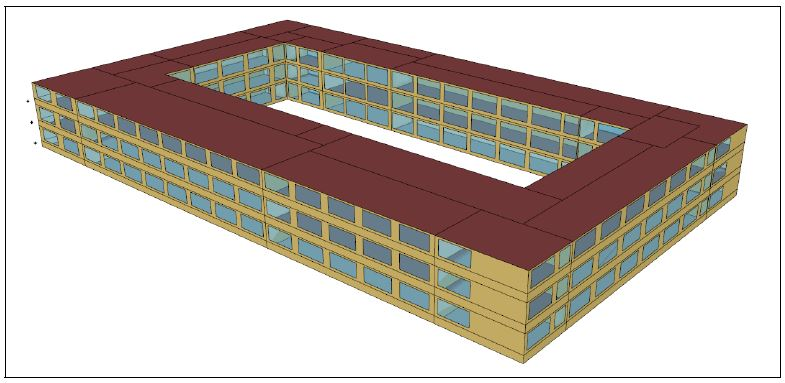
\includegraphics[scale=0.4]{Figures/building_model.jpg}
  \caption{Model of the building \cite{roman2015}}  
  \label{fig:building_model}
\end{figure}

\paragraph{Zoning map per floor} Figure \ref{fig:zoning} shows the room layout for a floor of the office building. It is divided into three different zones: meeting rooms (red), office areas (green) and border zones (blue). For every floor, the zoning is the same.

\begin{figure}[h!]
  \vspace{0.5em} %better style
  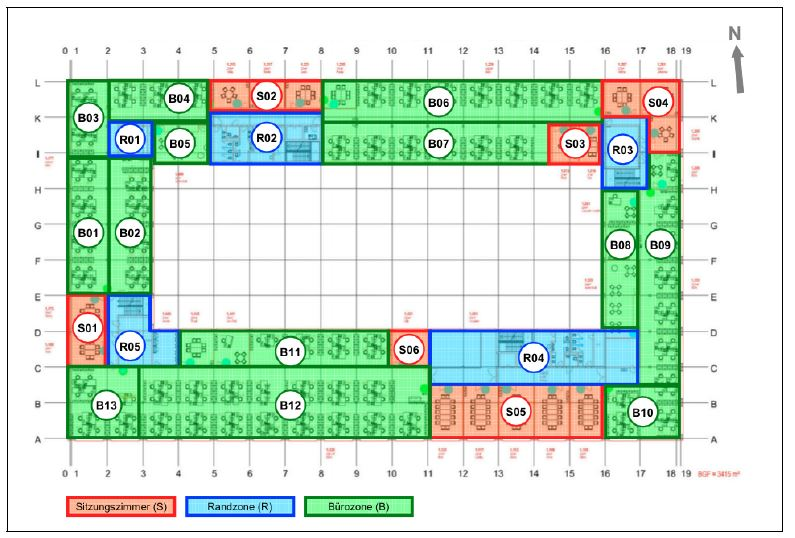
\includegraphics[scale=0.6]{Figures/zoning.jpg}
  \caption{Zoning for each floor \cite{roman2015}}  
  \label{fig:zoning}
\end{figure}

\paragraph{Mechanical Ventilation System} The studied building has two mechanical ventilation systems. The yellow area for the North-East zone and the blue area for the South-West zone (see figure \ref{fig:ventilation}). 

\begin{figure}[h!]
  \vspace{0.5em} %better style
  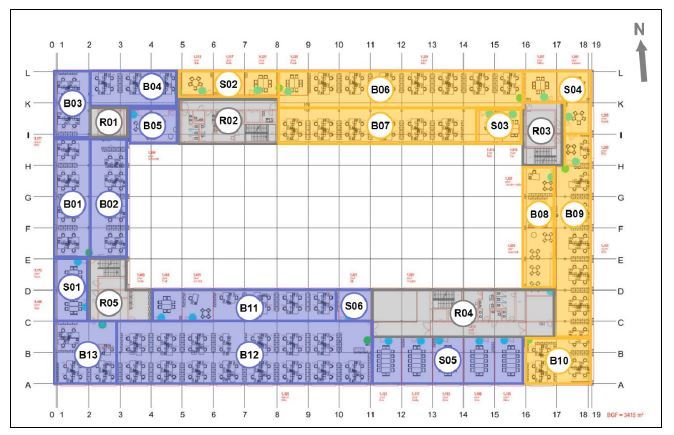
\includegraphics[scale=0.6]{Figures/ventilation.jpg}
  \caption{Mechanical ventilation systems per floor \cite{roman2015}}  
  \label{fig:ventilation}
\end{figure}

\paragraph{Heating and Cooling Systems} The studied building has two thermally-activated building systems (TABS). The red area for the North-East zone and the green area for the South-West zone (see figure \ref{fig:heating}). Each TABS supplies all floors of the corresponding building zone. There are some differences in the zoning of the mechanical ventilation systems and the heating and
cooling system. For example, room B10 is in the north/east zone of the ventilation system, but
in the south/west zone of the heating and cooling system.  

\begin{figure}[h!]
  \vspace{0.5em} %better style
  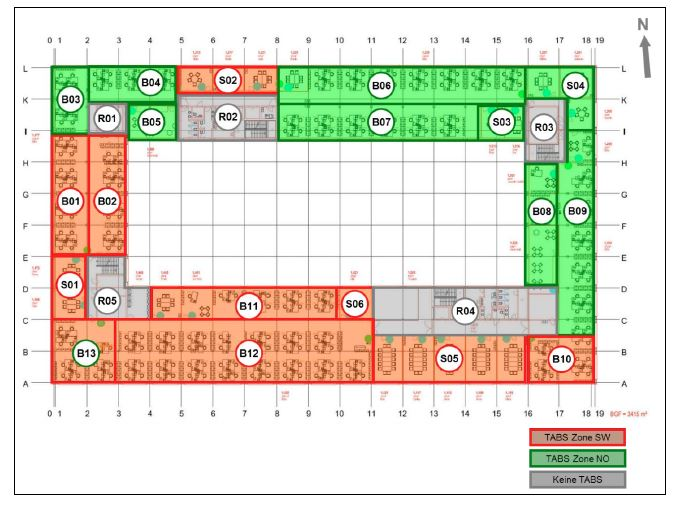
\includegraphics[scale=0.6]{Figures/heating.jpg}
  \caption{TAB systems per each floor \cite{roman2015}}  
  \label{fig:heating}
\end{figure}

\paragraph{Humidity and temperature in rooms}

Temperature and humidity are measured in 4 rooms of each floor. Therefore 12 variables named with the name of room are available in this dataset according to figure \ref{fig:temperature}.  

\begin{figure}[h!]
  \vspace{0.5em} %better style
  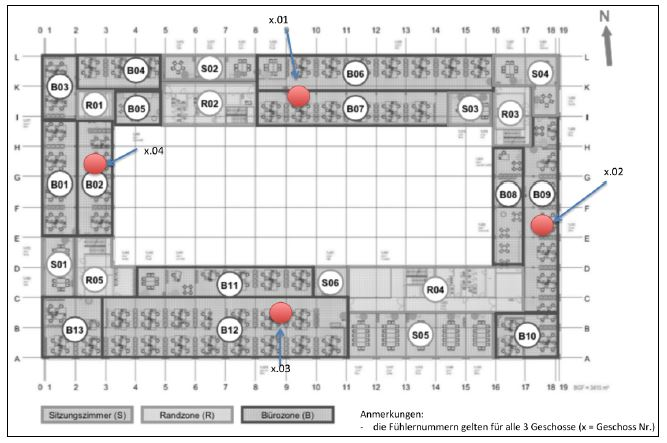
\includegraphics[scale=0.6]{Figures/temperature.jpg}
  \caption{Mechanical ventilation systems per floor \cite{roman2015}}  
  \label{fig:temperature}
\end{figure}


\section{Dataset handling}

The provided dataset has 64 variables with a time range of 3 years, from mid of 2012 until mid of 2015 with hourly time resolution. This implies 25943 registers per variable giving more than 1.6 million measurements. These 64 variables were associated according the provided information explained in section \ref{general_information}.  Table \ref{tab:variable_sum} summarizes the different categories of variables in the building dataset. The complete list of variables is included in the annex \ref{AppendixA}. Each category collects variables of the same type, same internal subsystems or that belong to the same spatial information zone according to section \ref{general_information}. Additionally, the dataset has been enriched with outdoor weather data. The buildings nearest weather station is Zurich-Kloten, for which the data has been acquired from the \textit{Bundesamt fur Meteorologie und Klimatologie Meteo Schweiz}. The variables are outdoor temperature (°C), precipitation (mm) and sunshine hours (min). More information about how the weather temperature changes in Switzerland is in  \cite{rebetez2008monthly}.
   
\begin{table}[htbp]
  \centering
  \scriptsize
  \caption{Variable categories within the Data-set}
    \begin{tabular}{|l|l|}
    \hline
    \multicolumn{1}{|c|}{\textbf{Variable name}} & \multicolumn{1}{c|}{\textbf{Unit}} \bigstrut\\
    \hline
    CO2 exhaust air & ppm \bigstrut\\
    \hline
    Humidity exhaust air & \% \bigstrut\\
    \hline
    Room humidity & \% \bigstrut\\
    \hline
    Temperature exhaust air & °C \bigstrut\\
    \hline
    Temperature intake air & °C \bigstrut\\
    \hline
    Room Temperature & °C \bigstrut\\
    \hline
    Outdoor Temperature & °C \bigstrut\\
    \hline
    Blinds status & 0/1 \bigstrut\\
    \hline
    Cooling TABS & kWh \bigstrut\\
    \hline
    Heating TABS & kWh \bigstrut\\
    \hline
    Sunshine presence per hour & minutes (min) \bigstrut\\
    \hline
    Precipitation level & mm \bigstrut\\
    \hline
    Blinds height & \% (100\% closed, 0\% open) \bigstrut\\
    \hline
    Blinds angle & \% (100\% closed, 0\% open) \bigstrut\\
    \hline
    \end{tabular}%
  \label{tab:variable_sum}%
\end{table}%



\subsection{Building Zones Category}
We divided the building dataset into coming from one of two main spatial zones in the building (i.e. North-East and South-West zone), according to the information provided by Synergy BTC AG. These zones are associated to two different mechanical ventilation and TABS systems. We associated each variable (i.e. time series of the measurements) to the according zone and created a metadata table that is included in \ref{sec:metadata_t}. Field \textit{breakout\_group} uses the codes $A\_\ast$ for the North-East zone and the codes $B\_\ast$ for the South-West zone. 
  
% Table generated by Excel2LaTeX from sheet 'Hoja6'
\begin{table}[htbp]
  \centering
  \scriptsize
  \caption{Extract of the proposed metadata table.}
    \begin{tabular}{|l|l|l|l|l|l|l|}
    \hline
    \rowcolor[rgb]{ 0,  0,  0} \textcolor[rgb]{ 1,  1,  1}{\textbf{tagname}} & \textcolor[rgb]{ 1,  1,  1}{\textbf{alias}} & \textcolor[rgb]{ 1,  1,  1}{\textbf{orientation}} & \textcolor[rgb]{ 1,  1,  1}{\textbf{category}} & \textcolor[rgb]{ 1,  1,  1}{\textbf{breakout\_group}} & \textcolor[rgb]{ 1,  1,  1}{\textbf{alias\_breakout\_group}} & \textcolor[rgb]{ 1,  1,  1}{\textbf{units}} \bigstrut\\
    \hline
    \rowcolor[rgb]{ .851,  .851,  .851} V005\_vent01\_CO2 & CO2 Ventilation NE & NE   & CO2  & A    & CO2 Ventilation NE & ppm \bigstrut\\
    \hline
    V022\_vent02\_CO2 & CO2 Ventilation SW & SW   & CO2  & B    & CO2 Ventilation SW & ppm \bigstrut\\
    \hline
    \rowcolor[rgb]{ .851,  .851,  .851} V037\_tabs\_cold\_SW & Cooling tabs SW & SW   & Cooling & B\_1 & Cooling SW & kWh \bigstrut\\
    \hline
    V075\_tabs\_cold\_NO & Cooling tabs NE & NE   & Cooling & A\_1 & Cooling NE & kWh \bigstrut\\
    \hline
    \rowcolor[rgb]{ .851,  .851,  .851} V034\_tabs\_warm\_SW & Heating tabs SW & SW   & Heating & B\_2 & Heating SW & kWh \bigstrut\\
    \hline
    \end{tabular}%
  \label{tab:Extarct of the Metadata}%
\end{table}%


\subsection{Building measures - Time Series}
\label{sec:dealing}
Script \ref{eq:script} shows how the time series are stored in the database. This script represents a register where variable is the key and the numeric value is the measure of the variable at time equal to timestamp. Our approach adopts a Big-Data database that uses JSON-like documents with schemas. Each register is a JSON document with keys like the timestamp, name of the variable, epoch\footnote{ Unix epoch (or Unix time or POSIX time or Unix timestamp) is the number of seconds that have elapsed since January 1, 1970 (midnight UTC/GMT), not counting leap seconds (in ISO 8601: 1970-01-01T00:00:00Z).}, and others. The flexibility and scalability that Big-Data offers, allows us to retrieve high volumes of data quickly and store complex structures like nested JSON objects. 

\begin{equation}
\scriptsize
\label{eq:script}
\begin{array}{llcl}
\{ &  &  &  \\ 
& timestamp & : & 2012-06-23 \quad 01:00:00 \\	
& epoch & : & 1340406000.0 \\	
 & variable1 & : & 142.25 	\\	
 & variable2 & : & 123.45 	\\	
 & ... &  &  	\\	
 & variablen & : & 123.45 	\\
\} & & & \\
\end{array}
\end{equation}

In our approach, we include the epoch time to the existing dataset to manipulate the time series. This is one simple way to query the time series using ranges of time in a time series dataset. For example, script \ref{scr:query} indicates a NOSQL expression \footnote{This is MongoDB syntax, manual available on \url{https://docs.mongodb.com/tutorials/}} for asking values of a time series within the time range defined by the key \textit{epoch}. \textit{db.timeseries} is the collection of JSON documents that contains the time series of the dataset. The reserved words \textit{\$gte, \$lte} define the time range (i.e. greater than equal to 1412204098 and lower than equal to 1412204099) of the requested variables \textit{variable\_1, ..., variable\_n}. 

\begin{equation}
\scriptsize
\label{scr:query}
\begin{array}{rlll}
db.timeseries.find(\{ &  &  &  	\\
	epoch : \{ &&  &			\\
		&  \$gte&:& 1412204098, 	\\
		&    \$lte&:& 1412204099 		\\
		& \}     \\
     	\},\{& & 						\\
	 variable\_1 & : & True, &		\\    
    	..., & &	&			\\
    	variable\_n & : &  True 		\\
    	\}) \\
\end{array}
\end{equation}

Another proposition from the last script uses a list of timestamps as is showed in script \ref{eq:script2}\footnote{One common framework that facilitates similar operations for manipulating the time series is included as \textit{rs\_common\_framework\_v4.py}.}. \textbf{An important remark} to do is that the NOSQL queries do not guarantee a chronological order of the requested elements by default. Methods to order the requested data are needed, this is a very important aspect to consider when one uses time series, especially for the training process as it is explained in section \ref{sec:cross}. 

\begin{equation}
\scriptsize
\label{eq:script2}
\begin{array}{rlll}
db.timeseries.find(\{ &  &  &  	\\
	timestamp : \{ &&  &			\\
		&  \$in &:& [$'2012-12-21', '2012-12-23', ...$], 	\\
		& \}     \\
     	\},\{& & 						\\
	 variable\_1 & : & True, &		\\    
    	..., & &	&			\\
    	variable\_n & : &  True 		\\
    	\}) \\
\end{array}
\end{equation}
 
Finally, we show in figure \ref{fig:big_data_example} an example of JSON objects stored in the Big-Data database. It shows the power of this approach where key/value pairs are nested. This provides flexibility to our data models, facilitating the storage and the retrieve of complex objects. 
  

\begin{figure}[h!]
  \vspace{0.5em} %better style
  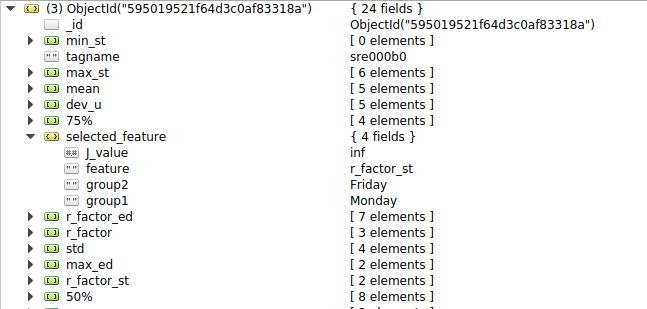
\includegraphics[scale=0.6]{Figures/DataBase_example.jpg}
  \caption{Example of JSON objects stored in the Big-Data database.}  
  \label{fig:big_data_example}
\end{figure}
